\documentclass[12pt,a4paper]{article}

\usepackage[utf8]{inputenc}
\usepackage[T1]{fontenc}
\usepackage[french]{babel}
\usepackage[a4paper,margin=2.5cm]{geometry}
\usepackage{amsmath}
\usepackage{amssymb}
\usepackage{booktabs}
\usepackage{graphicx}
\usepackage{float}
\usepackage{listings}
\usepackage{xcolor}
\usepackage{hyperref}

\graphicspath{{images/}}

\definecolor{codegray}{gray}{0.95}
\definecolor{codecomment}{rgb}{0.25,0.45,0.25}
\definecolor{codekeyword}{rgb}{0.20,0.25,0.60}

\lstset{
  language=Python,
  backgroundcolor=\color{codegray},
  basicstyle=\ttfamily\footnotesize,
  keywordstyle=\color{codekeyword}\bfseries,
  commentstyle=\color{codecomment},
  stringstyle=\color{red!55!black},
  breaklines=true,
  frame=single,
  rulecolor=\color{black!25},
  numbers=left,
  numberstyle=\tiny\color{black!50},
  showstringspaces=false,
  columns=fullflexible
}

\hypersetup{
  colorlinks=true,
  linkcolor=blue!50!black,
  urlcolor=blue!60!black,
  pdftitle={Détection d'anomalies par autoencodeur profond},
  pdfauthor={Achraf Errafai}
}

\begin{document}

\begin{titlepage}
  \centering
  \vspace*{1cm}
  {\Large \textbf{Université Cadi Ayyad}\par}
  \vspace{0.3cm}
  {\large École Nationale des Sciences Appliquées de Safi\par}
  \vspace{0.3cm}
  {\large Filière G.INFO et IDIA\par}
  \vfill
  {\Large Projet Intégrateur ERP\par}
  \vspace{0.5cm}
  {\Huge \textbf{Risque Systémique \& Early Warning System (CoVaR)}\par}
  \vspace{0.8cm}
  {\LARGE \textbf{Volet 4 : Intelligence Artificielle, Intégration \& Validation}\par}
  \vspace{0.5cm}
  {\Large Détection d'anomalies par autoencodeur profond\par}
  \vfill
  \begin{tabular}{ll}
    \textbf{Groupe 10} & \\
    CHAFIK Mouad & ERRAFAI Achraf \\
    MARZAQ Jihane & NADIR Safaa \\
    \textbf{Encadrant} & M. JRAIFI \\
    \textbf{Année universitaire} & 2026--2027
  \end{tabular}
  \vfill
\end{titlepage}

\tableofcontents
\clearpage

\section{Introduction et objectifs du volet IA}

Le projet \emph{Risque Systémique \& Early Warning System (CoVaR)} vise à construire une chaîne
quantitative et intégrable dans un environnement ERP pour surveiller les risques communs du
secteur bancaire. Le présent volet complète les indicateurs classiques de risque, notamment la
VaR, la CoVaR et la $\Delta\mathrm{CoVaR}$, par un mécanisme de détection non supervisée des
changements atypiques dans la structure de dépendance entre banques.

L'analyse porte sur cinq établissements : Attijariwafa Bank (ATW), Banque Centrale Populaire
(BCP), Bank of Africa (BOA), CIH Bank (CIH) et Crédit du Maroc (CDM). Les rendements et les
résidus standardisés issus des modèles GARCH alimentent l'estimation DCC-GARCH. Celle-ci produit,
pour chaque date, une matrice de corrélation conditionnelle dynamique. Une variation inhabituelle
de cette matrice peut précéder ou accompagner une période de tension systémique, même lorsque
les indicateurs marginaux de volatilité ne suffisent pas encore à déclencher une alerte.

L'objectif est donc de :
\begin{itemize}
  \item représenter chaque matrice DCC par ses corrélations hors diagonale uniques ;
  \item apprendre, sans étiquette de crise, la structure des observations considérées comme normales ;
  \item mesurer l'écart de reconstruction de chaque journée ;
  \item transformer cet écart en signal d'alerte précoce au moyen du quantile empirique à 99\,\%.
\end{itemize}

Les données utilisées dans le pipeline actif sont les données de marché locales normalisées dans
le répertoire canonique \texttt{data/real/}. Les données synthétiques historiques restent
distinctes et ne sont pas mélangées aux observations réelles.

\section{Formulation mathématique de l'autoencodeur}

\subsection{Vecteur d'entrée}

Pour $k=5$ banques, la matrice de corrélation DCC à la date $t$ est notée
$R_t=(\rho_{ij,t})_{1\leq i,j\leq k}$. Elle est symétrique et possède une diagonale unitaire.
La redondance de la partie inférieure est supprimée en conservant uniquement les éléments de la
partie triangulaire supérieure stricte :
\[
  \mathbf{x}_t =
  \left(
  \rho_{12,t},\rho_{13,t},\ldots,\rho_{45,t}
  \right)^\top
  \in \mathbb{R}^{k(k-1)/2}.
\]
Avec $k=5$, la dimension est :
\[
  d=\frac{5(5-1)}{2}=10.
\]

\subsection{Encodeur et décodeur}

L'autoencodeur est un réseau dense symétrique. L'encodeur applique successivement des couches
affines et une activation ReLU :
\[
  \mathbf{z}_t=f_{\theta}(\mathbf{x}_t)
  =\operatorname{ReLU}\!\left(
  W_e\mathbf{x}_t+\mathbf{b}_e
  \right),
\]
où $\mathbf{z}_t\in\mathbb{R}^{\ell}$ est la représentation latente et $\ell<d$. Dans
l'implémentation, la compression suit la structure $10\rightarrow 8\rightarrow 5\rightarrow 3$.

Le décodeur reconstruit le vecteur d'origine :
\[
  \widehat{\mathbf{x}}_t=g_{\phi}(\mathbf{z}_t)
  =W_d\mathbf{z}_t+\mathbf{b}_d,
\]
avec une architecture miroir $3\rightarrow 5\rightarrow 8\rightarrow 10$. Les activations ReLU
sont utilisées dans les couches cachées. La dernière couche est linéaire afin de reconstruire
directement les corrélations.

\subsection{Apprentissage et score d'anomalie}

L'apprentissage est non supervisé et utilise uniquement les observations du régime normal,
sélectionnées chronologiquement avant la période de validation. Les paramètres sont ajustés en
minimisant la perte quadratique moyenne :
\[
  \mathcal{L}(\theta,\phi)
  =\frac{1}{n}\sum_{t=1}^{n}
  \left\|\mathbf{x}_t-\widehat{\mathbf{x}}_t\right\|_2^2.
\]

Pour une observation quelconque, le score d'anomalie est son erreur de reconstruction :
\[
  s_t=\operatorname{MSE}(\mathbf{x}_t,\widehat{\mathbf{x}}_t)
  =\frac{1}{d}\sum_{j=1}^{d}
  (x_{t,j}-\widehat{x}_{t,j})^2.
\]
Une journée est signalée lorsque son score dépasse le seuil empirique :
\[
  \tau_{0.99}=Q_{0.99}\left(\{s_t:t\in\mathcal{T}_{\mathrm{normal}}\}\right),
  \qquad
  \mathrm{Alerte}_t=\mathbb{1}_{\{s_t>\tau_{0.99}\}}.
\]
Ce choix limite théoriquement le taux de faux positifs à environ 1\,\% sur la distribution
d'apprentissage, sans imposer une loi paramétrique au score.

\section{Architecture logicielle et validation}

\subsection{Module \texttt{src/ml.py}}

Le module Python centralise les responsabilités suivantes :
\begin{itemize}
  \item extraction des dix corrélations uniques à partir d'un tenseur de matrices DCC ;
  \item définition du modèle \texttt{CorrelationAutoencoder} en PyTorch ;
  \item entraînement par Adam et perte MSE ;
  \item reconstruction des observations et calcul vectorisé des scores ;
  \item sélection automatique du processeur CPU lorsque la carte graphique locale n'est pas
        compatible avec les noyaux CUDA du paquet installé.
\end{itemize}

L'extrait suivant résume l'interface utilisée par le prototype :

\begin{lstlisting}
features = upper_triangle_features(dcc.correlations)
model = CorrelationAutoencoder(
    input_dim=10, latent_dim=3, hidden_dims=(8, 5)
)
training = train_autoencoder(
    train_features,
    model=model,
    epochs=150,
    batch_size=32,
    learning_rate=1e-3,
    device="cpu",
)
scores = training.model.score(all_features)
threshold = np.percentile(
    training.model.score(train_features), 99.0
)
\end{lstlisting}

\subsection{Prototype Notebook IA}

Le notebook \texttt{notebooks/05\_ia\_anomaly\_detection.ipynb} charge les données réelles
canoniques, reconstruit la chaîne GARCH--DCC-GARCH, puis effectue une séparation temporelle.
Les 70 premiers pour cent constituent la fenêtre de développement. Les observations connues comme
stressées sont exclues de l'apprentissage normal lorsqu'elles sont disponibles. La
standardisation des dix caractéristiques est calculée exclusivement sur cette fenêtre normale,
afin d'éviter une fuite d'information vers la validation.

Le notebook produit trois vues complémentaires :
\begin{enumerate}
  \item la convergence de la perte MSE pendant les 150 époques ;
  \item la distribution transversale des erreurs avec le seuil au 99e percentile ;
  \item l'évolution temporelle du score et les alertes dépassant le seuil.
\end{enumerate}

\subsection{Tests unitaires}

Le fichier \texttt{tests/test\_ml.py} vérifie notamment :
\begin{itemize}
  \item la dimension $(n,10)$ du vecteur extrait pour cinq banques ;
  \item la dimension $(n,10)$ de la reconstruction ;
  \item l'obtention d'un score par observation ;
  \item le rejet des matrices d'entrée de dimension incorrecte ou non finies.
\end{itemize}

Ces tests sont complétés par les tests du chargeur de données réelles dans
\texttt{tests/test\_real\_data.py}. La suite complète du dépôt a été validée avec pytest.

\section{Résultats expérimentaux et analyse graphique}

\subsection{Convergence de l'apprentissage}

\begin{figure}[H]
  \centering
  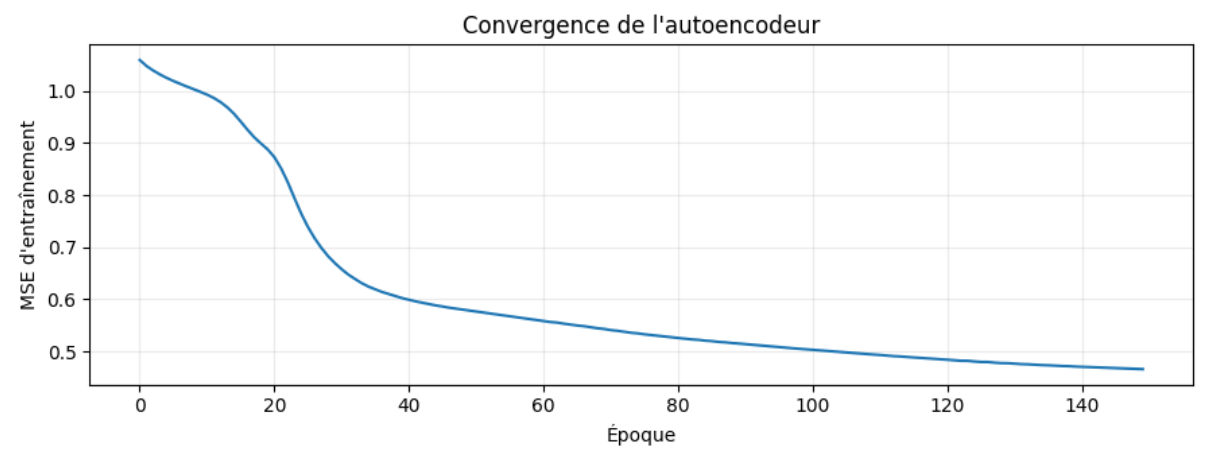
\includegraphics[width=\textwidth]{convergence_autoencodeur.png}
  \caption{Convergence de l'autoencodeur (MSE d'entraînement sur 150 époques)}
  \label{fig:convergence}
\end{figure}

La figure~\ref{fig:convergence} montre une décroissance lisse de la MSE d'entraînement,
d'environ $1{,}06$ au début à environ $0{,}47$ après 150 époques. L'absence d'oscillation
marquée suggère une optimisation stable avec le taux d'apprentissage choisi. La perte ne doit
cependant pas être interprétée comme une probabilité de crise : elle mesure uniquement la
capacité du réseau à reproduire la structure de corrélation apprise sur le régime normal.

\subsection{Distribution des erreurs et seuil d'alerte}

\begin{figure}[H]
  \centering
  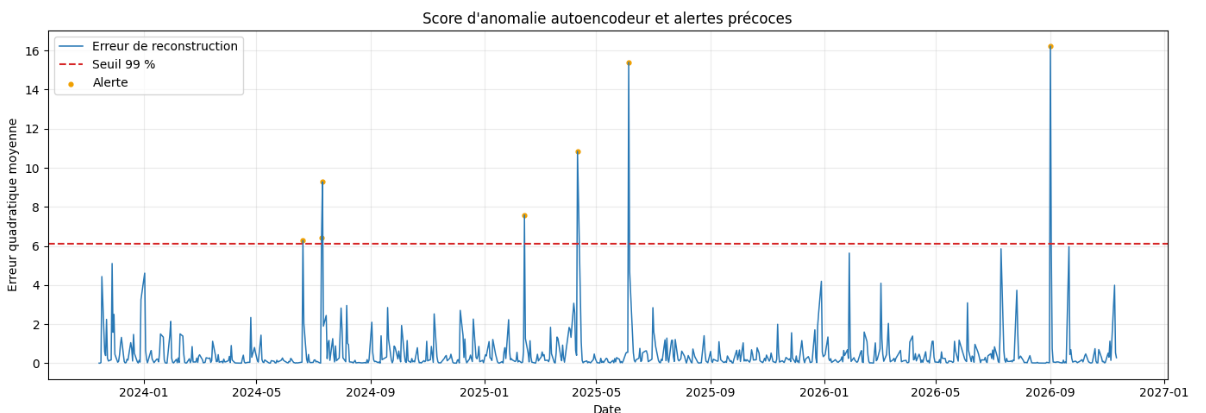
\includegraphics[width=\textwidth]{distribution_erreurs.png}
  \caption{Distribution des erreurs de reconstruction et seuil d'alerte au 99e percentile}
  \label{fig:distribution}
\end{figure}

La figure~\ref{fig:distribution} présente une distribution fortement asymétrique à droite :
la majorité des observations possède une erreur proche de zéro, tandis qu'une minorité
d'observations se situe dans une queue éloignée. La ligne verticale rouge en tirets représente
le seuil empirique du 99e percentile, situé autour de
$\mathrm{MSE}\simeq 5{,}9$. Les observations à droite de cette ligne sont candidates à une
alerte. Cette règle est robuste à une distribution non gaussienne et s'adapte à l'échelle
effective des erreurs normales.

\subsection{Évolution temporelle et alertes précoces}

\begin{figure}[H]
  \centering
  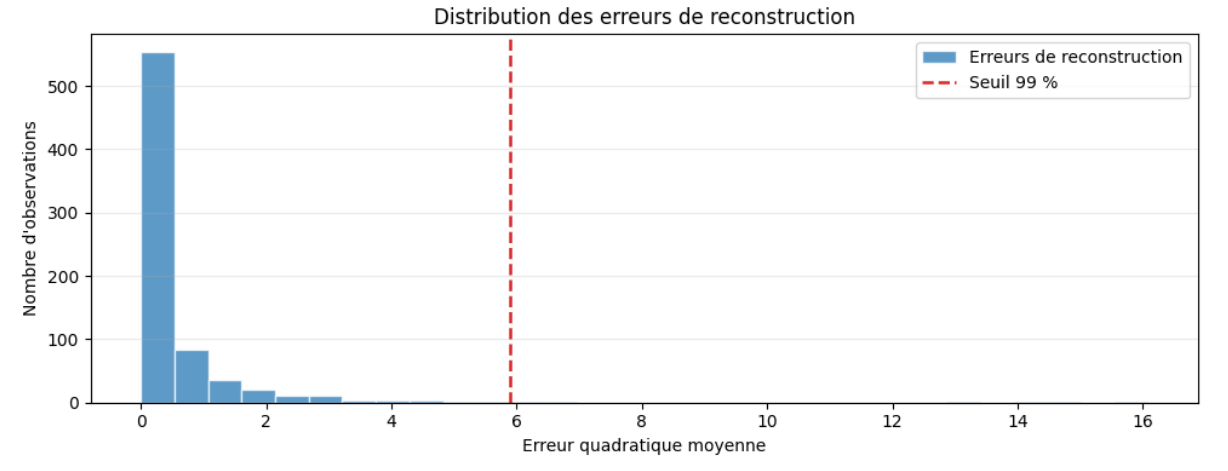
\includegraphics[width=\textwidth]{score_anomalie_alertes.png}
  \caption{Score d'anomalie de l'autoencodeur et alertes précoces au-dessus du seuil 99\,\%}
  \label{fig:score}
\end{figure}

La figure~\ref{fig:score} montre un niveau de reconstruction généralement faible sur la ligne de
base, ponctué de pics distincts. Les marqueurs orange correspondent aux dates dont le score
dépasse la ligne rouge en tirets. Plusieurs pics atteignent approximativement $9$ à plus de
$16$, ce qui traduit une rupture nette avec la structure de dépendance apprise durant le régime
normal.

L'axe horizontal couvre la période allant de la fin de l'année 2023 à la fin de l'année 2026.
Cette lecture temporelle doit respecter les fenêtres du jeu canonique du projet : les dates des
matrices DCC, des rendements et des indicateurs de risque doivent être alignées avant toute
comparaison avec VaR, CoVaR ou $\Delta\mathrm{CoVaR}$. Une alerte d'autoencodeur n'est pas, à
elle seule, une preuve de crise ; elle constitue un signal complémentaire qui doit être
confirmé par la volatilité, les corrélations, les pertes extrêmes et le contexte économique.

\section{Conclusion et intégration dans l'ERP Odoo}

Le volet IA apporte une couche de surveillance non supervisée centrée sur la dépendance
conditionnelle entre les cinq banques. Le choix du vecteur triangulaire réduit la redondance des
matrices DCC, tandis que l'autoencodeur apprend une représentation compacte de la structure
normale. Le score MSE fournit une mesure continue et facilement historisable ; son quantile à
99\,\% fournit une règle d'alerte explicite et reproductible.

Le dépôt contient actuellement l'addon Odoo \texttt{cours\_derives/}. Les fonctionnalités Early
Warning pourront être ajoutées dans cet addon ou dans un module complémentaire dépendant. Les
étapes d'intégration proposées sont les suivantes :
\begin{enumerate}
  \item créer un modèle métier d'alerte contenant la date, le score, le seuil, le niveau et la
        source de données ;
  \item importer périodiquement les scores calculés par le pipeline Python ;
  \item exposer dans une vue liste et une vue graphique les scores, les dépassements et les
        banques concernées par la fenêtre DCC ;
  \item combiner le score d'anomalie avec VaR, CoVaR et $\Delta\mathrm{CoVaR}$ dans une règle de
        criticité multi-indicateurs ;
  \item conserver l'explication de l'alerte : score observé, seuil, date de référence et
        version du modèle.
\end{enumerate}

Une évolution importante sera le suivi de la dérive du modèle. Le seuil et l'autoencodeur
devront être réévalués lorsque la distribution des corrélations changera durablement. La
traçabilité des versions, la séparation entre données réelles et données simulées, ainsi que la
validation humaine des alertes restent indispensables avant toute utilisation opérationnelle.

\end{document}
